\chapter{Krav}
I det følgende afsnit er der beskrevet de Use Cases, der har været udarbejdet ifm. udviklingen af systemet. Use Casene beskriver de anvendelsesmuligheder hver af de to typer af brugere har i systemet, hhv. Superbruger og Ekspedient.\\
Disse Use Cases bliver anvendt som kravsspecifikation for systemet, da de viser de reelle anvendelsesmuligheder. Ønskes yderligere specifikationer om disse use cases, henvises til dokumentationen, afsnit 1 - Kravspecifikation.

\section{Aktørbeskrivelse}

I det følgende afsnit kan der læses om de aktører, der er tilknyttet systemet. \\

\begin{figure}[H]
	\centering
	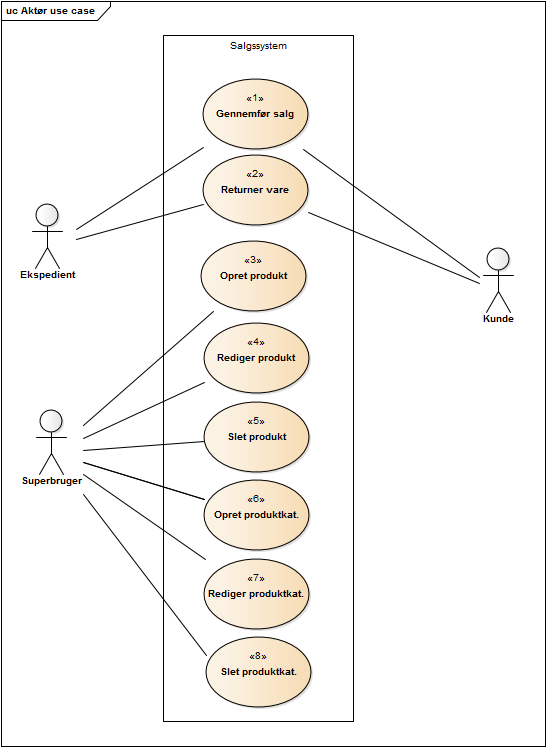
\includegraphics[width=0.6\textwidth]{Krav/Images/AktorUC}
	\caption{Use Cases med aktører}
	\label{fig:ActorUC}
\end{figure}

\begin{table}[H]
	\label{EKS}
	\begin{tabularx}{\textwidth}{|l|X|}
		\hline
		\textbf{Navn} & Ekspedient \\
		\hline
		\textbf{Type} & Primær \\
		\hline
		\textbf{Beskrivelse} & Ekspedient er en primær bruger af systemet, som benytter systemet til at sælge og returnere varer. \\
		\hline
	\end{tabularx}
	\captionsetup{justification=raggedright,singlelinecheck=false}
	\caption{Aktørbeskrivelse af Ekspedient}
	\label{tab:AktEks}
\end{table}


\begin{table}[H]
	\begin{tabularx}{\textwidth}{|l|X|}
		\hline
		\textbf{Navn} & Superbruger \\
		\hline
		\textbf{Type} & Primær \\
		\hline
		\textbf{Beskrivelse} & Superbruger er en primær bruger af systemet, som benytter systemet til at oprette, slette og redigere i systemets varekatalog. \\
		\hline
	\end{tabularx}
	\captionsetup{justification=raggedright,singlelinecheck=false}
	\caption{Aktørbeskrivelse af Superbruger}
	\label{tab:AktSuu}
\end{table}

\begin{table}[H]
	\label{KD}
	\begin{tabularx}{\textwidth}{|l|X|}
		\hline
		\textbf{Navn} & Kunde \\
		\hline
		\textbf{Type} & Sekundær \\
		\hline
		\textbf{Beskrivelse} & Kunden er en sekundær bruger af systemet, og ønsker at købe/returnere en eller flere varer igennem Ekspedient. Ekspedient er beskrevet i tabel \ref{tab:AktEks}.   \\
		\hline
	\end{tabularx}
	\captionsetup{justification=raggedright,singlelinecheck=false}
	\caption{Aktørbeskrivelse af Kunde}
	\label{tab:AktKu}
\end{table}

\section{Use Case beskrivelser}

I det følgende afsnit kan der læses om de Use Cases der er udarbejdet til systemet. Ønskes der yderligere specifikationer om disse usecases henvises der til dokumentationen, afsnit 1.5. \\

\subsubsection{Use Case 1 - Gennemfør salg}


\subsubsection{Use Case 2 - Returner vare}
Denne use case har til formål at returnere vare. Ekspedient indtaster varer til retur og trykker på knappen til returnering af varer. Herefter bliver der sendt informationer om returneringen til CentralServer.
\subsubsection{Use Case 3 - Opret produkt}
Denne Use Case har til formål at oprette et produkt i databasen. Oprettelse af produkter foregår på Administrationssystemet. Systemet betjenes af en Superbruger. Superbrugeren trykker på knappen til at oprette produkt og indtaster informationer om det nye produkt i det vindue der åbner. Informationerne er navnet på produktet, varenummer, pris og hvilken kategori produktet hører til. Når Superbruger godkender oprettelsen bliver der sendt besked til CentralServer om det nye produkt. Herefter lukker vinduet til at oprette produkt og det nye produkt kommer frem i den korrekte produktkategori.
\subsection{Use case 3: Opret \gls{PD}} \label{prodkat}
At oprette en \gls{PD}er til systemet.



\begin{table}[H]
\begin{tabularx}{\textwidth}{|l|X|}
\hline
\textbf{Navn}					& Opret \gls{PD} \\\hline
\textbf{Formål}					& \gls{SB} opretter \gls{PD} . \\\hline
\textbf{Initialisering}			& \gls{SB} \\\hline
\textbf{Aktører}				& \gls{SB} (Primær)\\\hline
\textbf{Reference}				& Ingen \\\hline
								
\textbf{Samtidige forekomster}	& $\infty$ \\\hline
\textbf{Prækondition}			& Der er oprettet forbindelse til \gls{CS}.
\\\hline
\textbf{Postkondition}			& Der er oprettet et nyt, tidligere ubenyttet \gls{PD} i systemet.
\\\hline
\textbf{Hovedscenarie}			& 1. \gls{SB} trykker på opret \gls{PD} på i \gls{AS}.\\												& 2. Et pop up vindue åbnes i \gls{GUI}, hvori der indtastes informationer om \gls{PD}et.\\
								& 3. \gls{SB} trykker på gem.\\
								& ~ [Ext 1: \gls{PD} eksisterer allerede] \\
								& 2. Systemet sender kommando til \gls{CS}.\\
								& ~ [Ext 2: \gls{CS} melder fejl.\\
								& 3. \gls{AS} modtager opdatering om nyt \gls{PD}. \\
								& 4. \gls{AS} opdaterer \gls{PD}listen \\\hline

\textbf{Extensions}						
								& [Ext 1: \gls{PD}et eksisterer allerede] \\
								& ~ 1. Beskedboks informerer \gls{SB} om at \gls{PD} allerede eksisterer.\\
								& ~ 2. Der fortsættes fra punkt 1.\\
									
								& [Ext 2: \gls{CS} melder fejl] \\
								& ~ 1. Beskedboks informerer \gls{SB} om fejl. \\
								& ~ 2. Usecasen afsluttes \\\hline
\end{tabularx}
\caption{Use case 3: Usecase for opret \gls{PD} }
\label{tab:UCop}
\end{table}

\subsubsection{Use Case 5 - Slet produkt}
Denne use case har til formål at slette et produkt fra produktkataloget. Superbruger vælger det produkt, der ønskes at slettes og trykker på knappen til slet, hvorefter et vindue præsenteres for Superbruger, hvori der bekræftes. Alternativt kan Superbruger højreklikke på produktet og følge samme fremgangsmåde. Efter endt use case er produktet slettet fra produktkataloget.
\subsection{Use case 5: Slet produkt}


\begin{table}[H]
\begin{tabularx}{\textwidth}{|l|X|}
\hline
\textbf{Navn}					& Slet produkt \\\hline
\textbf{Formål}					& At slette et produkt \\\hline
\textbf{Initialisering}			& \gls{SB} \\\hline
\textbf{Aktører}				& \gls{SB} \\\hline
\textbf{Reference}				& Ingen. \\\hline								
\textbf{Samtidige forekomster}	& $\infty$ \\\hline
\textbf{Prækondition}			& Der skal være et produkt at slette. \\\hline
\textbf{Postkondition}			& Det valgte produkt skal være slettet. \\
\hline
\textbf{Hovedscenarie}			& 1. \gls{SB} vælger det produkt der ønskes slettet, og trykker på knappen til at slette produkt.\\												
								& 2. Et dialogvindue, der spørger om produktet ønskes slettet, vises på skærmen.\\
								& 3. \gls{SB} trykker på knappen til at godkende sletningen og dialogvinduet forsvinder.\\
								& ~ [Ext 1: \gls{SB} vælger at annullere sletningen.]\\
								& 4. Produktet slettets umiddelbart herefter fra listen over produkt.\\
								& ~ [Ext 2: \gls{CS} melder fejl]\\
\hline
\textbf{Extensions}				& [Ext 1: \gls{SB} vælger at annullere sletningen.]\\
								& ~ 1. \gls{SB} trykker på knappen til at annullere sletningen.\\
								& ~ 2. Dialogvinduet forsvinder og intet yderligere foretages.\\
								& [Ext 2: \gls{CS} melder fejl] \\
								& ~ 1. Beskedboks informerer \gls{SB} om fejl. \\
								& ~ 2. Usecasen afsluttes \\\hline
\hline
\end{tabularx}
\caption{Use case 5: Slet produkt}
\label{tab:UCsp}
\end{table}
\subsubsection{Use Case 7 - Rediger produktkategori}
Denne Use Case har til formål at redigere navnet på en produktkategori i produktkataloget. For at udføre denne use case vælger Superbruger den ønskede produktkategori og trykker på knappen til redigering af produktkategori. Herefter præsenteres Superbruger med et vindue med oplysningerne på produktkategorien, hvori Superbruger retter navnet. Efter endt use case er produktkategorien redigeret i produktkataloget.
\subsubsection{Use Case 8 - Slet produktkategori}